\chapter{Image reconstruction}
\label{ch:image-reconstruction}

\begingroup
\raggedbottom

The goal is a single two-dimensional image from an aberrated FLFM acquisition. The method combines views by aligning and averaging them, as in classical light-field rendering \cite{levoyHanrahanLightFieldRendering2023}, and uses the FLFM design and notation of Guo et al. \cite{guo2019fourierLightField} without their forward model. It assumes a nominally two-dimensional fluorescent scene, corresponding structure visible in enough views, shifts within the search bounds, and a suitable central reference. It is not deconvolution, learned reconstruction, or scattering inversion, and it recovers neither a wavefront nor a three-dimensional object. Chapter~\ref{ch:experimental-setup} describes view extraction.

Let $V_{ij}(y,x)$ be view $(i,j)$ of an $N\times N$ grid, with $i,j\in\{1,\ldots,N\}$ and row--column position $(y,x)$ on the $H\times W$ pixel grid $\Omega$. In the global stage, the central view $V_{cc}$ is the reference. Pixels below a fraction of each image's own maximum are set to zero to form matching copies $\widetilde R^g$ and $\widetilde V_{ij}$, which reduces the influence of noise and defocused light. Cross-correlation over a bounded range of integer shifts $s$ gives one translation for each entire view,

\begin{equation}
    d^g_{ij}=\operatorname*{arg\,max}_{s}\sum_{(y,x)\in\Omega}\widetilde R^g(y,x)\,\widetilde V_{ij}(y-s_y,x-s_x).
\end{equation}

Translating the original, unthresholded views by $d^g_{ij}$ gives the aligned views $V^g_{ij}$, whose mean $G=N^{-2}\sum_{i,j}V^g_{ij}$ is the intermediate global-stage average.

A single translation cannot follow displacements that vary across a view, so the local stage uses $G$ as the reference for every aligned view. At each pixel, a bounded search, possibly in steps finer than one pixel, selects the displacement $d^\ell_{ij}(y,x)$ with the strongest Gaussian-smoothed, intensity-normalized match between thresholded copies of $G$ and $V^g_{ij}$. This score is not standard normalized cross-correlation, and each pixel is chosen independently. The unthresholded aligned view is sampled backward at the displaced location, and the mean over all views is the final rectified image,

\begin{equation}
    V^\ell_{ij}(y,x)=\operatorname{Interp}\!\left(V^g_{ij},(y,x)-d^\ell_{ij}(y,x)\right),
    \qquad I_{\mathrm{rect}}(y,x)=\frac{1}{N^2}\sum_{i=1}^{N}\sum_{j=1}^{N}V^\ell_{ij}(y,x).
\end{equation}

Figure~\ref{fig:single-view-alignment} follows one noncentral view through both stages. Each sampling arrow starts at an output position and points to the source location read in that stage. The full pipeline is sketched in Figure~\ref{fig:reconstruction-sequence} (Appendix~\ref{app:reconstruction-method}). Because $G$ and $I_{\mathrm{rect}}$ average the same views at successive stages, comparing them within one run isolates what local refinement adds.

Both averages weight all $N^2$ views equally, including alignment's zero borders, and each view contributes to its own local reference. Nothing measures match confidence or enforces invertibility or intensity conservation, so a sharper feature may reflect better alignment, geometric compression, or merged structures. Appendix~\ref{app:reconstruction-method} gives the defaults, exact local score, and handling of ties and degenerate scores.

\begin{figure}[p]
    \centering
    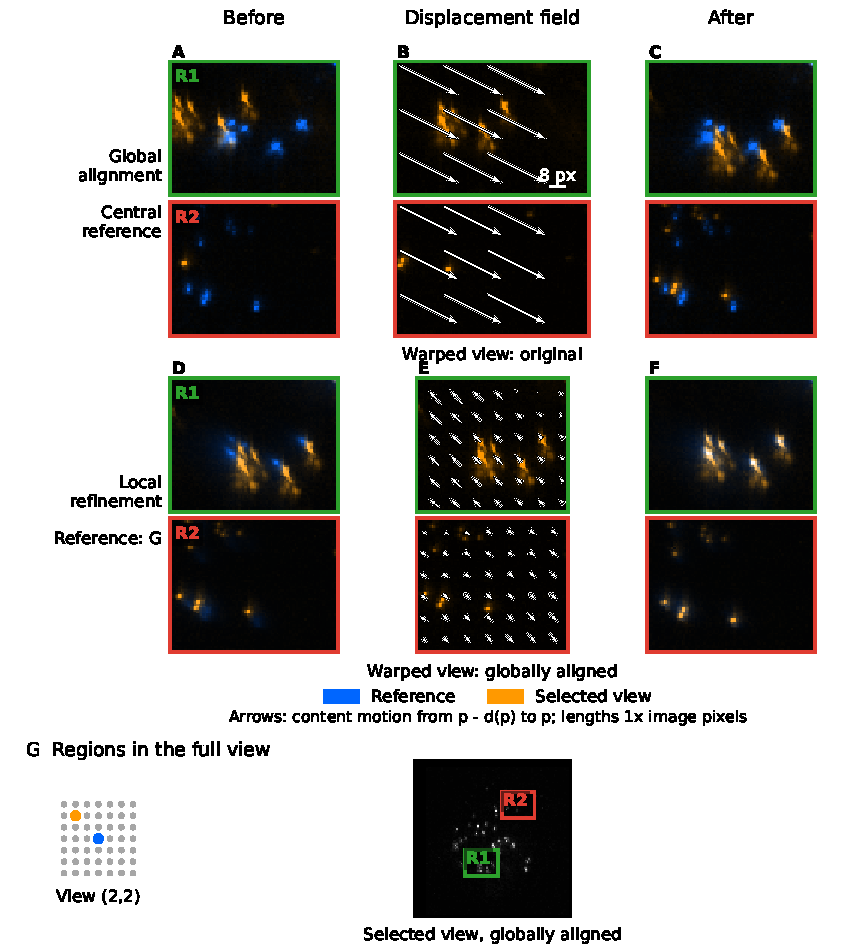
\includegraphics[width=\linewidth]{figures/ch05/alignment-evolution.pdf}
    \caption[Image evolution and backward sampling through both alignment stages.]{Image evolution and backward sampling for view $(2,2)$ in a $7\times7$ FLFM acquisition of fluorescent beads under gel eyedrops (dense10 run; one-based view indices). (A--C) Global alignment uses the original central reference. (D--F) Local refinement uses the global-stage average $G$, including the selected view. The left and right columns overlay the reference (blue) and selected view (orange) before and after correction; C and D contain the same aligned view with different references. Middle panels show grayscale references and arrows from output positions $p$ toward source locations $p-d(p)$ in the original view (B) or globally aligned view (E). Lengths use image pixels; arrows leaving the crop are omitted. (G) The marked output pixel reads intensity at $p_{\mathrm{src}}=p-d^\ell(p)$ in the source patch. Here $p=(262,167)$ and $p_{\mathrm{src}}=(267,172)$ in zero-based row--column coordinates. The dashed arrow denotes lookup. All images share linear display limits and use nearest-neighbor display; reconstruction uses linear interpolation. The crop and marker are illustrative.}
    \label{fig:single-view-alignment}
\end{figure}

\clearpage
\endgroup
